\documentclass[11pt]{article}
\usepackage[fleqn]{amsmath}\textwidth 6.5in
\oddsidemargin -0.25in
%\evensidemargin -0.5in
\topmargin -0.25in
\textheight 9.0in

\newcommand{\docname}{\bf wvs-074r7}
\newcommand{\docdate}{22 May 2019}

\usepackage{graphicx}

\usepackage{floatflt}

\ifx\pdfoutput\undefined
  \pdfoutput=0
  \usepackage[hypertex,plainpages,hyperindex=true]{hyperref}
  \hypersetup{%
    hypertexnames=false%
  }
  % Specify the driver for the color package
  \ExecuteOptions{dvips}
  %\ExecuteOptions{xdvi}
\else
  \ifnum\pdfoutput>0
    \usepackage[pdftex,plainpages,hyperindex=true,pdfpagelabels]{hyperref}
    \hypersetup{%
      hypertexnames=false,%
      colorlinks=true,%
      linktocpage=true,%
    }
    % Specify the driver for the color package
    \ExecuteOptions{pdftex}
  \else
    \usepackage[hypertex,plainpages,hyperindex=true]{hyperref}
    \hypersetup{%
      hypertexnames=false%
    }
    % Specify the driver for the color package
    \ExecuteOptions{dvips}
    %\ExecuteOptions{xdvi}
  \fi
\fi

\begin{document}

%\tracingcommands=1
\newlength{\hW} % heading box width
\newlength{\pW} % page number field width
\settowidth{\hW}{\docname}
\settowidth{\pW}{Page \pageref{lastpage}\ of \pageref{lastpage}}
\ifdim \pW > \hW \setlength{\hW}{\pW} \fi
\makeatletter
\def\@biblabel#1{#1.}
\newcommand{\ps@twolines}{%
  \renewcommand{\@oddhead}{%
    \docdate\hfill\parbox[t]{\hW}{{\hfill\docname}\newline
                          Page \thepage\ of \pageref{lastpage}}}%
\renewcommand{\@evenhead}{}%
\renewcommand{\@oddfoot}{}%
\renewcommand{\@evenfoot}{}%
}%
\makeatother
\pagestyle{twolines}

\vspace{-10pt}
\begin{tabbing}
\phantom{References: }\= \\
To: \>Van\\
Subject: \>Tangent heights and angles for scattering calculations\\
From: \>Van Snyder\\
References: \>wvs-068, wvs-070, wvs-071\\
\end{tabbing}

\parindent 0pt \parskip 8pt
\vspace{-20pt}

\newcommand{\pC}{{\bfseries\sffamily C}}
\newcommand{\pO}{{\bfseries\sffamily O}}
\newcommand{\pP}{{\bfseries\sffamily P}}

We wish to calculate paths to \pP\ at various angles, along which
radiation arriving at \pP\ would be scattered toward an observer at \pO. 
Ultimately, this radiation will be convolved with the scattering phase
function at \pP\ to calculate radiation scattered at \pP\ in the
direction of \pO, but that is the subject of memos wvs-068, wvs-070 and
wvs-071.

Consider first the case when rays do not reflect from the Earth's surface. 

\ifnum\pdfoutput>0
{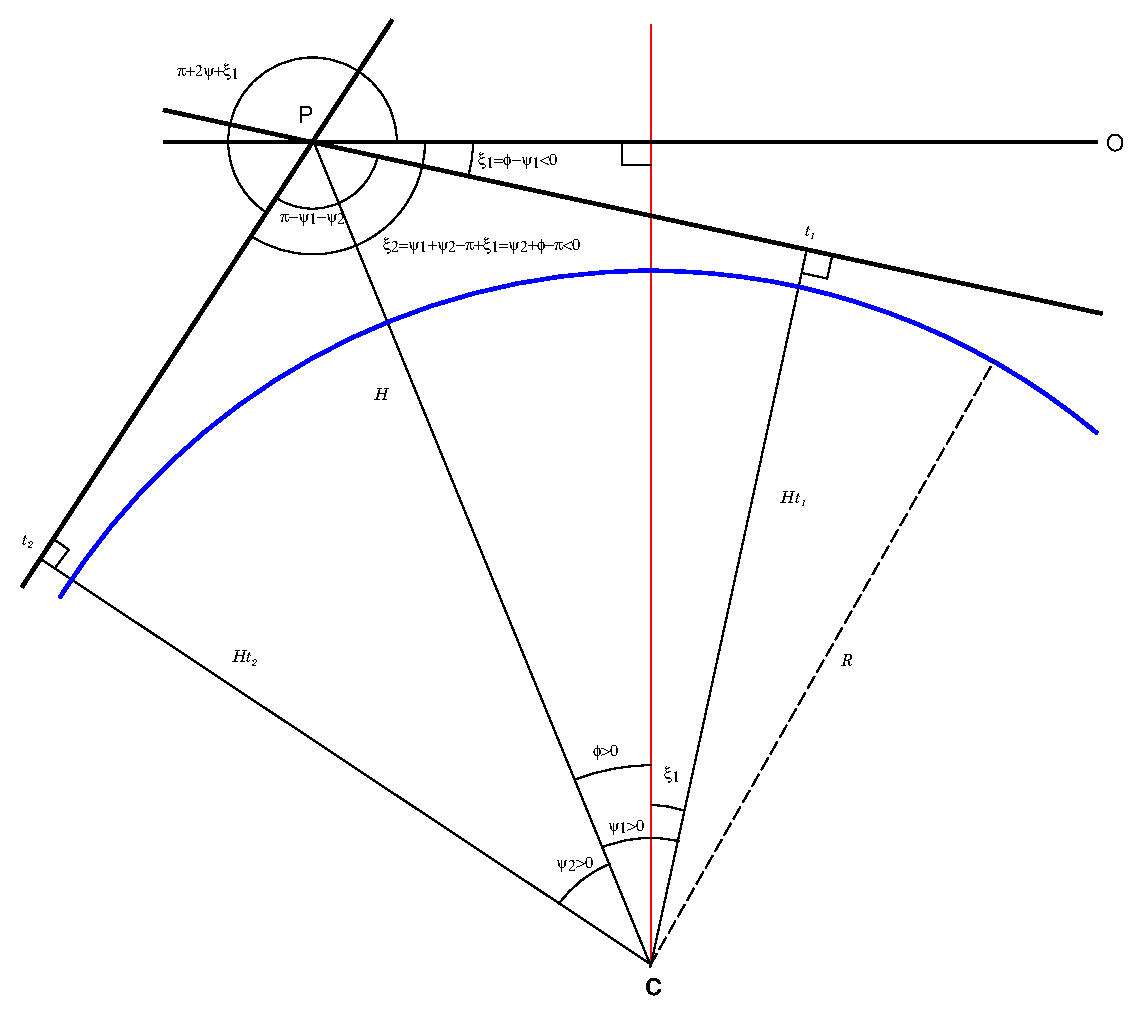
\includegraphics[width=450pt,height=500pt,clip=true,keepaspectratio=true,
viewport=20 126 553 600]{./wvs-074-scatter-1}}
\else
{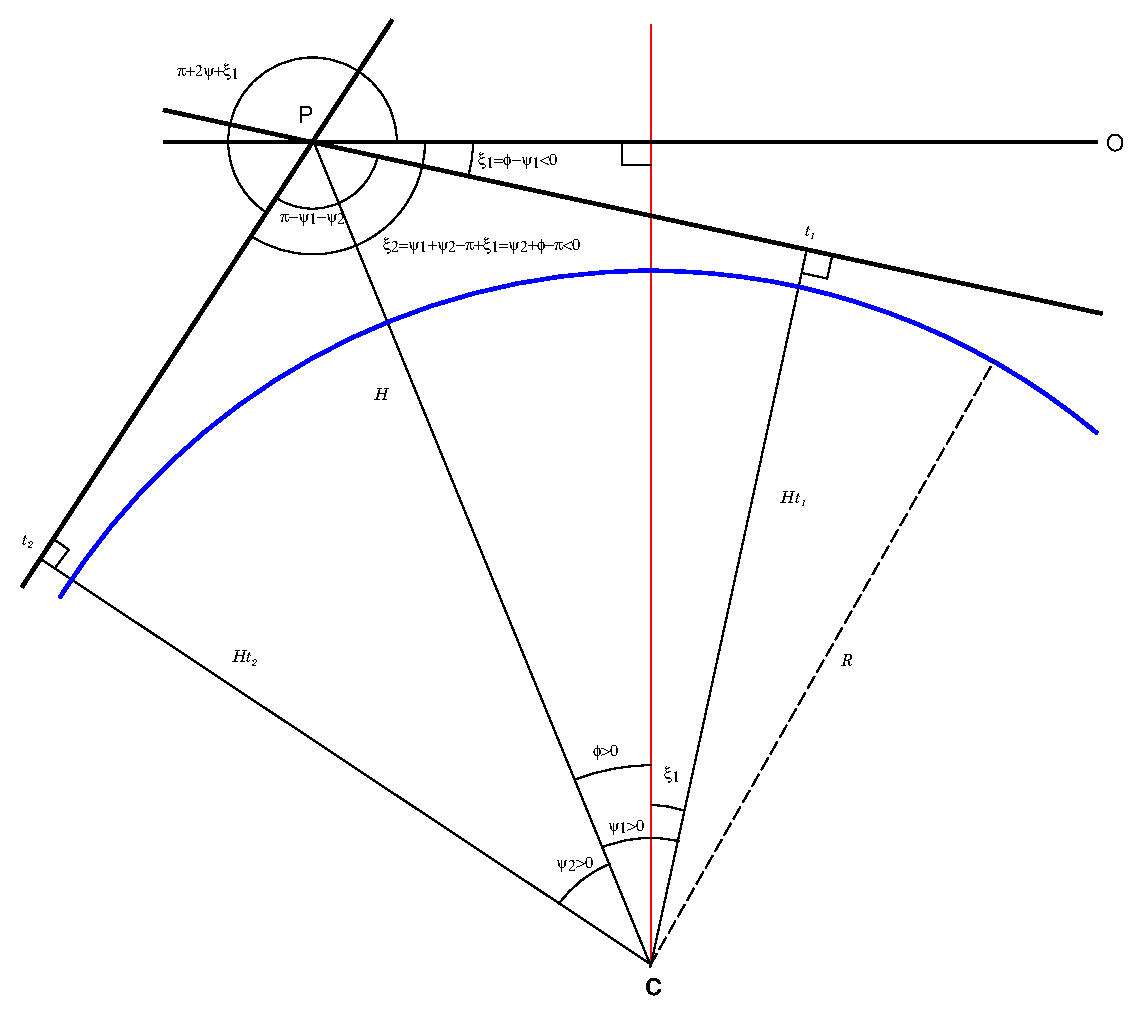
\includegraphics[width=450pt,height=500pt,clip=true,keepaspectratio=true,
bb=20 126 553 600]{./wvs-074-scatter-1}}
\fi

We wish to calculate the angles $\xi_1$ and $\xi_2$ with respect to the
horizon defined by the line \pP\pO, to characterize rays along which to
calculate radiative transfer to \pP\ at specified coordinates $(H,\phi)$,
where $H$ is height measured from the center \pC\ of the equivalent
circular earth and $\phi$ is the angle at \pC\ measured anti-clockwise
from the reference (red) line, which is normal to the horizon and passes
through the center of the equivalent circular Earth.  The angles $\xi_1$
and $\xi_2$ at \pP\ between the ray and the line \pP\pO, measured
anti-clockwise at \pP\ from the horizon, are calculated from $H,\,\phi$,
and the tangent heights $Ht_1$ and $Ht_2$ at the tangent points $t_1$ and
$t_2$, which in turn are calculated from specified log pressure $\zeta$
using hydrostatic equilibrium.  Although $\zeta$ is the same at $t_1$ and
$t_2$, $Ht_1$ and $Ht_2$ are not necessarily equal because of the
possibility of different temperature profiles below $t_1$ and $t_2$.  In
any case, neither $Ht_1$ nor $Ht_2$ exceeds $H$.

Radiation can arrive at \pP\ along two rays that pass through $t_1$ and
$t_2$. Along one ray the angle at \pP\ is $\xi_1$, and along the other it
is $\xi_2$.  Radiation can arrive at \pP\ along opposite rays, that would
pass through $t_1$ and $t_2$ if they continued past \pP, at angles
$\pi+\xi_1$ and $\pi+\xi_2$.

The angle $\psi_1 = \angle t_1$\pC\pP\ at \pC\ between lines to the limb
ray tangent point $t_1$ and the scattering point \pP\ is
%
\begin{equation}
  \psi_1 = \cos^{-1} \frac{Ht_1}{H} \,.
\end{equation}
%
and similarly for the angle $\psi_2 = \angle$\pP\pC$t_2$.  The value of
$\xi_1$ at which a ray arriving at \pP\ from the direction nearest to \pO\
is tangent to the Earth's surface is denoted $\xi_c$ (not shown in the
figure).  If $|\xi_1| > |\xi_c|$, the ray is an earth-intersecting ray,
described below.  The value of $\xi_c$ is
%
\begin{equation}
%  \xi_c = -\left(\frac\pi2 - \phi - \psi(R) \right)\,,\,\,
   \xi_c = \phi - \psi(R)\,,\,\,
    \phi-\frac\pi2 \leq \xi_c \leq 0\,,\,\,\psi(R) = \cos^{-1} \frac{R}H\,,
\end{equation}
%
where $R$ is the radius of the equivalent circular earth.  The angle
$\xi_1$ below the horizon of the ray arriving at \pP\ from the direction
nearer to \pO\ is
%
\begin{equation}
  \xi_1 = \phi - \psi_1\,,\,\, \xi_c \leq \xi_1 \leq 0\,.
\end{equation}
%
The angle $\xi_2$ below the horizon of the ray arriving at \pP\ from the
direction opposite \pO\ is
%
\begin{equation}
  \xi_2 = \psi_1 + \psi_2 - \pi + \xi_1 = \psi_2 + \phi-\pi\,,\,\,
    -\pi \leq \xi_2 \leq -2 \psi(R) + \xi_c\,.
\end{equation}
%
If we assume $Ht_1 = Ht_2$, that is, the same equivalent circular earth is
sufficiently accurate at both limb tangent angles, this becomes
%
\begin{equation}
  \xi_2 = \psi_1 + \phi-\pi\,,\,\,
    -\pi \leq \xi_2 \leq -2 \psi(R) + \xi_c = 
      -\left(\frac\pi2 - \phi + \psi(R) \right)\,.
\end{equation}
%
The angles at \pC\ from the reference line to the tangent points $t_1$
and $t_2$ are $\xi_1$ and $\psi_1+\psi_2+\xi_1 = \pi+\xi_2$, respectively
(remember that $\xi_1$ is negative in the figure).

\newpage

Consider now the case when rays reflect from the Earth's surface ($|\xi_3| >
|\xi_c|$).

\ifnum\pdfoutput>0
{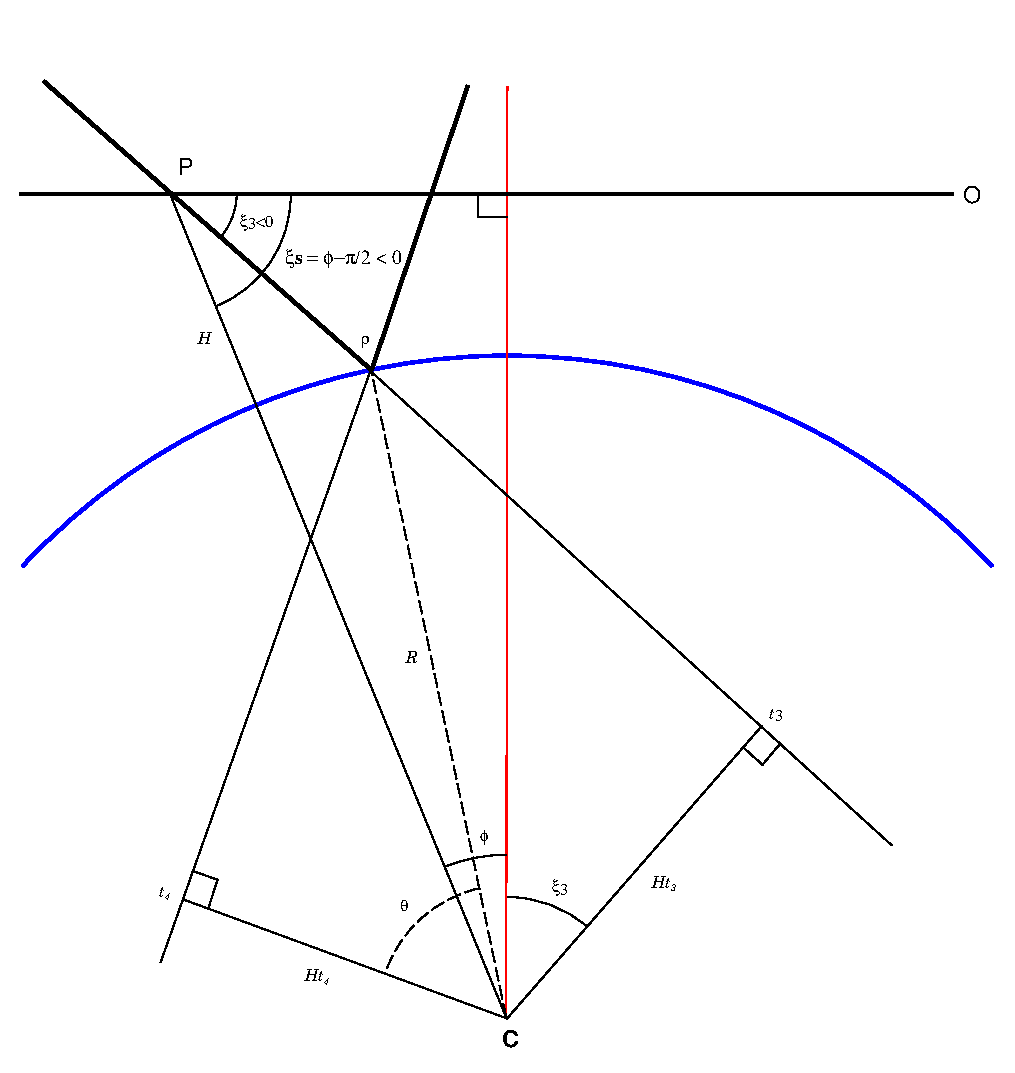
\includegraphics[width=450pt,height=500pt,clip,clip=true,keepaspectratio=true,
viewport=89 126 560 625]{./wvs-074-scatter-2}}
\else
{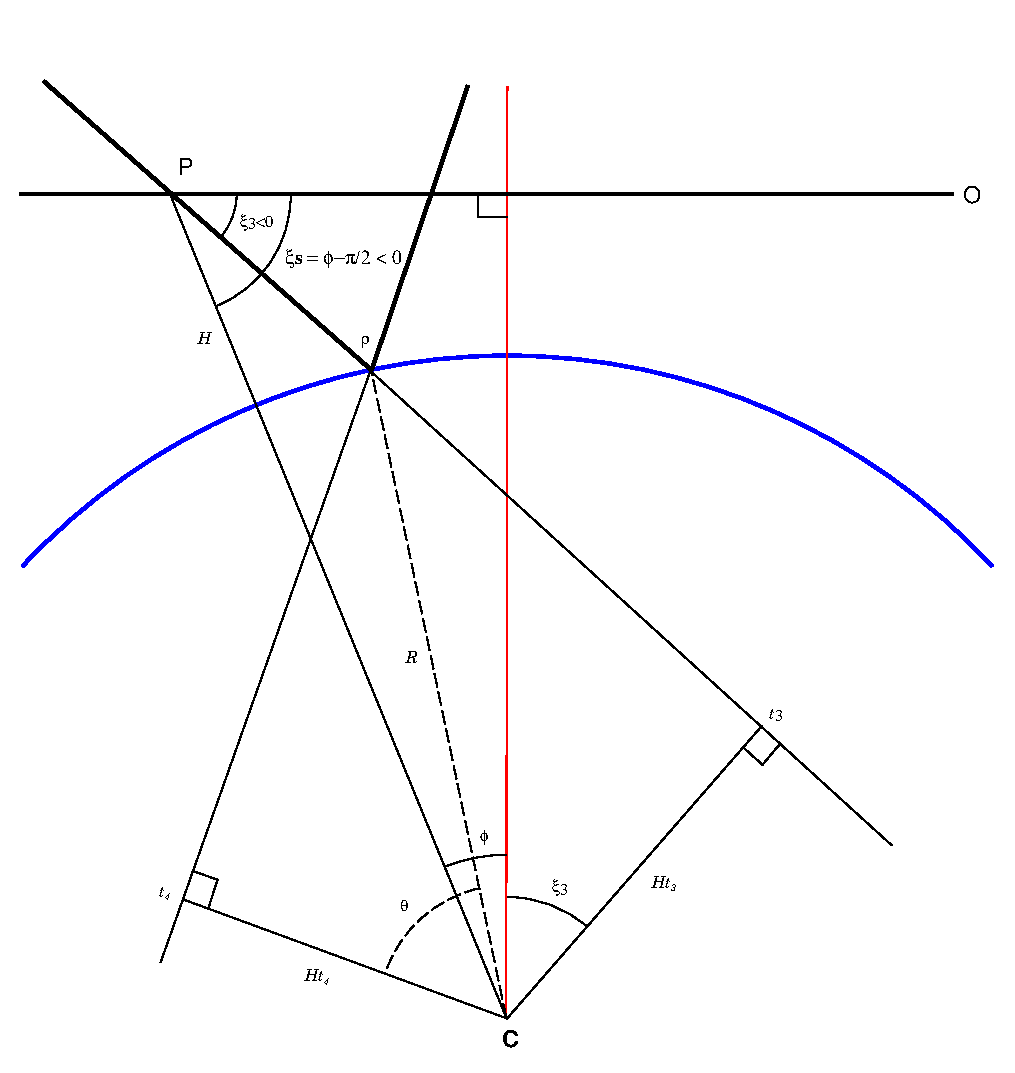
\includegraphics[width=450pt,height=500pt,clip,clip=true,keepaspectratio=true,
bb=89 126 560 625]{./wvs-074-scatter-2}}
\fi

The tangent point for a ray reflected from the Earth's surface would be
below the surface.  Therefore the height cannot be specified by $\zeta$
and hydrostatic equilibrium.  Rather $\xi_3$ is specified and $Ht_3 =
Ht_4$ is calculated:
%
\begin{equation}
  Ht_3 = H | \cos(\phi-\xi_3)|\,,
\end{equation}
%
The angle $\theta = \angle t_4$\pC$\rho$ at \pC\ between the rays to the
reflection point $\rho$ and $t_4$ is
%
\begin{equation}
  \theta = \cos^{-1} \frac{Ht_4}R \,.
\end{equation}
%
and the angle $\angle t_3$\pC$\rho$ has the same magnitude. The angle at
\pC\ between rays to the direct and scattered ray tangents $t_3$ and
$t_4$ is therefore $2 \theta$.

The angles at \pC\ from the reference line to the rays to the tangent
points $t_3$ and $t_4$ are $\xi_3$ and $2\theta+\xi_3$, respectively.

The same formulae are valid when $\xi_3 < -\phi$, that is, when the
incident ray arrives at $\rho$ from the direction opposite to the
direction from \pP\ to \pO.

\label{lastpage}
\end{document}

% $Id$

% $Log$
% Revision 1.8  2013/06/04 00:54:24  vsnyder
% Correct mistake Igor found in equation for xi_c
%
% Revision 1.7  2013/03/28 19:16:25  vsnyder
% Improve wording as Igor suggested
%
% Revision 1.6  2013/03/25 22:53:44  vsnyder
% Improve exposition and graphics
%
% Revision 1.5  2012/10/23 02:01:26  vsnyder
% Correct some typos
%
% Revision 1.4  2012/03/30 20:41:42  vsnyder
% Repair graphics stuff
%
% Revision 1.3  2009/09/17 18:27:11  vsnyder
% Typo
%
% Revision 1.2  2009/07/29 03:08:53  vsnyder
% R2
%
